% Options for packages loaded elsewhere
\PassOptionsToPackage{unicode}{hyperref}
\PassOptionsToPackage{hyphens}{url}
\PassOptionsToPackage{dvipsnames,svgnames,x11names}{xcolor}
%
\documentclass[
  number,
  3p]{elsarticle}

\usepackage{amsmath,amssymb}
\usepackage{iftex}
\ifPDFTeX
  \usepackage[T1]{fontenc}
  \usepackage[utf8]{inputenc}
  \usepackage{textcomp} % provide euro and other symbols
\else % if luatex or xetex
  \usepackage{unicode-math}
  \defaultfontfeatures{Scale=MatchLowercase}
  \defaultfontfeatures[\rmfamily]{Ligatures=TeX,Scale=1}
\fi
\usepackage{lmodern}
\ifPDFTeX\else  
    % xetex/luatex font selection
\fi
% Use upquote if available, for straight quotes in verbatim environments
\IfFileExists{upquote.sty}{\usepackage{upquote}}{}
\IfFileExists{microtype.sty}{% use microtype if available
  \usepackage[]{microtype}
  \UseMicrotypeSet[protrusion]{basicmath} % disable protrusion for tt fonts
}{}
\makeatletter
\@ifundefined{KOMAClassName}{% if non-KOMA class
  \IfFileExists{parskip.sty}{%
    \usepackage{parskip}
  }{% else
    \setlength{\parindent}{0pt}
    \setlength{\parskip}{6pt plus 2pt minus 1pt}}
}{% if KOMA class
  \KOMAoptions{parskip=half}}
\makeatother
\usepackage{xcolor}
\setlength{\emergencystretch}{3em} % prevent overfull lines
\setcounter{secnumdepth}{5}
% Make \paragraph and \subparagraph free-standing
\ifx\paragraph\undefined\else
  \let\oldparagraph\paragraph
  \renewcommand{\paragraph}[1]{\oldparagraph{#1}\mbox{}}
\fi
\ifx\subparagraph\undefined\else
  \let\oldsubparagraph\subparagraph
  \renewcommand{\subparagraph}[1]{\oldsubparagraph{#1}\mbox{}}
\fi


\providecommand{\tightlist}{%
  \setlength{\itemsep}{0pt}\setlength{\parskip}{0pt}}\usepackage{longtable,booktabs,array}
\usepackage{calc} % for calculating minipage widths
% Correct order of tables after \paragraph or \subparagraph
\usepackage{etoolbox}
\makeatletter
\patchcmd\longtable{\par}{\if@noskipsec\mbox{}\fi\par}{}{}
\makeatother
% Allow footnotes in longtable head/foot
\IfFileExists{footnotehyper.sty}{\usepackage{footnotehyper}}{\usepackage{footnote}}
\makesavenoteenv{longtable}
\usepackage{graphicx}
\makeatletter
\def\maxwidth{\ifdim\Gin@nat@width>\linewidth\linewidth\else\Gin@nat@width\fi}
\def\maxheight{\ifdim\Gin@nat@height>\textheight\textheight\else\Gin@nat@height\fi}
\makeatother
% Scale images if necessary, so that they will not overflow the page
% margins by default, and it is still possible to overwrite the defaults
% using explicit options in \includegraphics[width, height, ...]{}
\setkeys{Gin}{width=\maxwidth,height=\maxheight,keepaspectratio}
% Set default figure placement to htbp
\makeatletter
\def\fps@figure{htbp}
\makeatother

\makeatletter
\makeatother
\makeatletter
\makeatother
\makeatletter
\@ifpackageloaded{caption}{}{\usepackage{caption}}
\AtBeginDocument{%
\ifdefined\contentsname
  \renewcommand*\contentsname{Table of contents}
\else
  \newcommand\contentsname{Table of contents}
\fi
\ifdefined\listfigurename
  \renewcommand*\listfigurename{List of Figures}
\else
  \newcommand\listfigurename{List of Figures}
\fi
\ifdefined\listtablename
  \renewcommand*\listtablename{List of Tables}
\else
  \newcommand\listtablename{List of Tables}
\fi
\ifdefined\figurename
  \renewcommand*\figurename{Figure}
\else
  \newcommand\figurename{Figure}
\fi
\ifdefined\tablename
  \renewcommand*\tablename{Table}
\else
  \newcommand\tablename{Table}
\fi
}
\@ifpackageloaded{float}{}{\usepackage{float}}
\floatstyle{ruled}
\@ifundefined{c@chapter}{\newfloat{codelisting}{h}{lop}}{\newfloat{codelisting}{h}{lop}[chapter]}
\floatname{codelisting}{Listing}
\newcommand*\listoflistings{\listof{codelisting}{List of Listings}}
\makeatother
\makeatletter
\@ifpackageloaded{caption}{}{\usepackage{caption}}
\@ifpackageloaded{subcaption}{}{\usepackage{subcaption}}
\makeatother
\makeatletter
\@ifpackageloaded{tcolorbox}{}{\usepackage[skins,breakable]{tcolorbox}}
\makeatother
\makeatletter
\@ifundefined{shadecolor}{\definecolor{shadecolor}{rgb}{.97, .97, .97}}
\makeatother
\makeatletter
\makeatother
\makeatletter
\makeatother
\journal{Science}
\ifLuaTeX
  \usepackage{selnolig}  % disable illegal ligatures
\fi
\usepackage[]{natbib}
\bibliographystyle{elsarticle-num}
\IfFileExists{bookmark.sty}{\usepackage{bookmark}}{\usepackage{hyperref}}
\IfFileExists{xurl.sty}{\usepackage{xurl}}{} % add URL line breaks if available
\urlstyle{same} % disable monospaced font for URLs
\hypersetup{
  pdftitle={Response to West et al.~(2023)},
  pdfauthor={Hugh A. Graham; Andrew M. Cunliffe; Edward T.A. Mitchard; Javier Ruiz Ramos; Leonardo Sáenz; David F.R.P. Burslem; Christopher Philipson},
  colorlinks=true,
  linkcolor={blue},
  filecolor={Maroon},
  citecolor={Blue},
  urlcolor={Blue},
  pdfcreator={LaTeX via pandoc}}

\setlength{\parindent}{6pt}
\begin{document}

\begin{frontmatter}
\title{Response to West et al.~(2023)}
\author[1,2]{Hugh A. Graham%
\corref{cor1}%
}
 \ead{hugh.graham@permianglobal.com} 
\author[2]{Andrew M. Cunliffe%
%
}

\author[3]{Edward T.A. Mitchard%
%
}

\author[1]{Javier Ruiz Ramos%
%
}

\author[1]{Leonardo Sáenz%
%
}

\author[4]{David F.R.P. Burslem%
%
}

\author[1]{Christopher Philipson%
\corref{cor1}%
}
 \ead{christopher.philipson@permianglobal.com} 

\affiliation[1]{organization={Permian Global Research
Ltd.},addressline={3 Cavendish Square},city={London},postcode={W1G
0LB},postcodesep={}}
\affiliation[2]{organization={University of Exeter, Geography, Faculty
of Environment, Science and Economy},,postcodesep={}}
\affiliation[3]{organization={Space Intelligence Ltd.},addressline={93
George Street},city={Edinburgh},postcode={EH2 3ES},postcodesep={}}
\affiliation[4]{organization={University of Aberdeen, School of
Biological Sciences},city={Aberdeen},postcode={AB24 3UU},postcodesep={}}

\cortext[cor1]{Corresponding author}







        





\end{frontmatter}
    \ifdefined\Shaded\renewenvironment{Shaded}{\begin{tcolorbox}[frame hidden, sharp corners, breakable, interior hidden, boxrule=0pt, enhanced, borderline west={3pt}{0pt}{shadecolor}]}{\end{tcolorbox}}\fi

Avoided Deforestation Conservation Projects (ADCP) must deliver carbon
emission reductions and necessitate comparisons between observations in
protected forests and counterfactual scenarios
\citep{balmford_realizing_2023}. West et al. \citep{west_action_2023}
used the synthetic control (SC) method to choose pools of controls with
similar covariate structure to ADCPs. SCs were calculated from the mean
deforestation rate of pools, weighted by covariate similarity with the
project. We agree SC could improve the evaluation of ADCP. However, SC
are also vulnerable to ``gaming'' or bias through inappropriate donor
pool design/sampling and require refinement
\citep{balmford_realizing_2023} before they can improve upon existing
ADCP approaches.

West et al. \citep{west_action_2023} claim that most ADCPs overestimate
avoided deforestation or do not significantly reduce deforestation.
These conclusions are poorly supported by their analysis because:

\begin{itemize}
\item
  The implemented SC approach can suffer from bias
  \citep{abadie_using_2021} due to substantial and incompatible
  differences between deforestation drivers, forest type and
  (bio)geography that are not adequately captured. Important covariates
  are ignored, such as distance to roads and rivers
  \citep{laurance_roads_2017, barber_roads_2014}, fire risk
  \citep{amador-jimenez_unintended_2020}, or indicators of forest
  structure \citep{duncanson_aboveground_2022} that predict biomass,
  timber value and logging effort. Using the authors' code, we extracted
  the locations of controls used to create the SC for project-856
  (Figure~\ref{fig-map}), located in Colombia's Pacific-montane-forest.
  No weighted donors were in the same political jurisdiction or
  ecoregion as the project and the highest weighted donor (0.46) was in
  the Amazon, 900 km away.
\item
  Calculations derived from Global Forest Change (GFC)
  \citep{hansen_quantification_2010} inherit known sensitivity and
  accuracy issues
  \citep{kinnebrew_biases_2022, galiatsatos_assessment_2020}. It is
  inappropriate to compare GFC-based calculations with those reported by
  projects, which are better calibrated for local contexts, because
  meaningful comparisons require deforestation rates to be derived using
  identical methods. Further, it is accepted that GFC is inappropriate
  for site-level deforestation assessment, in isolation
  \citep{galiatsatos_assessment_2020, bos_global_2019}.
\item
  West et al. \citep{west_action_2023} do not demonstrate that SC
  counterfactuals are more accurate than project methods, undermining
  their ability to interpret differences between the SC and
  project-reported deforestation rates.
\end{itemize}

\begin{figure}

{\centering 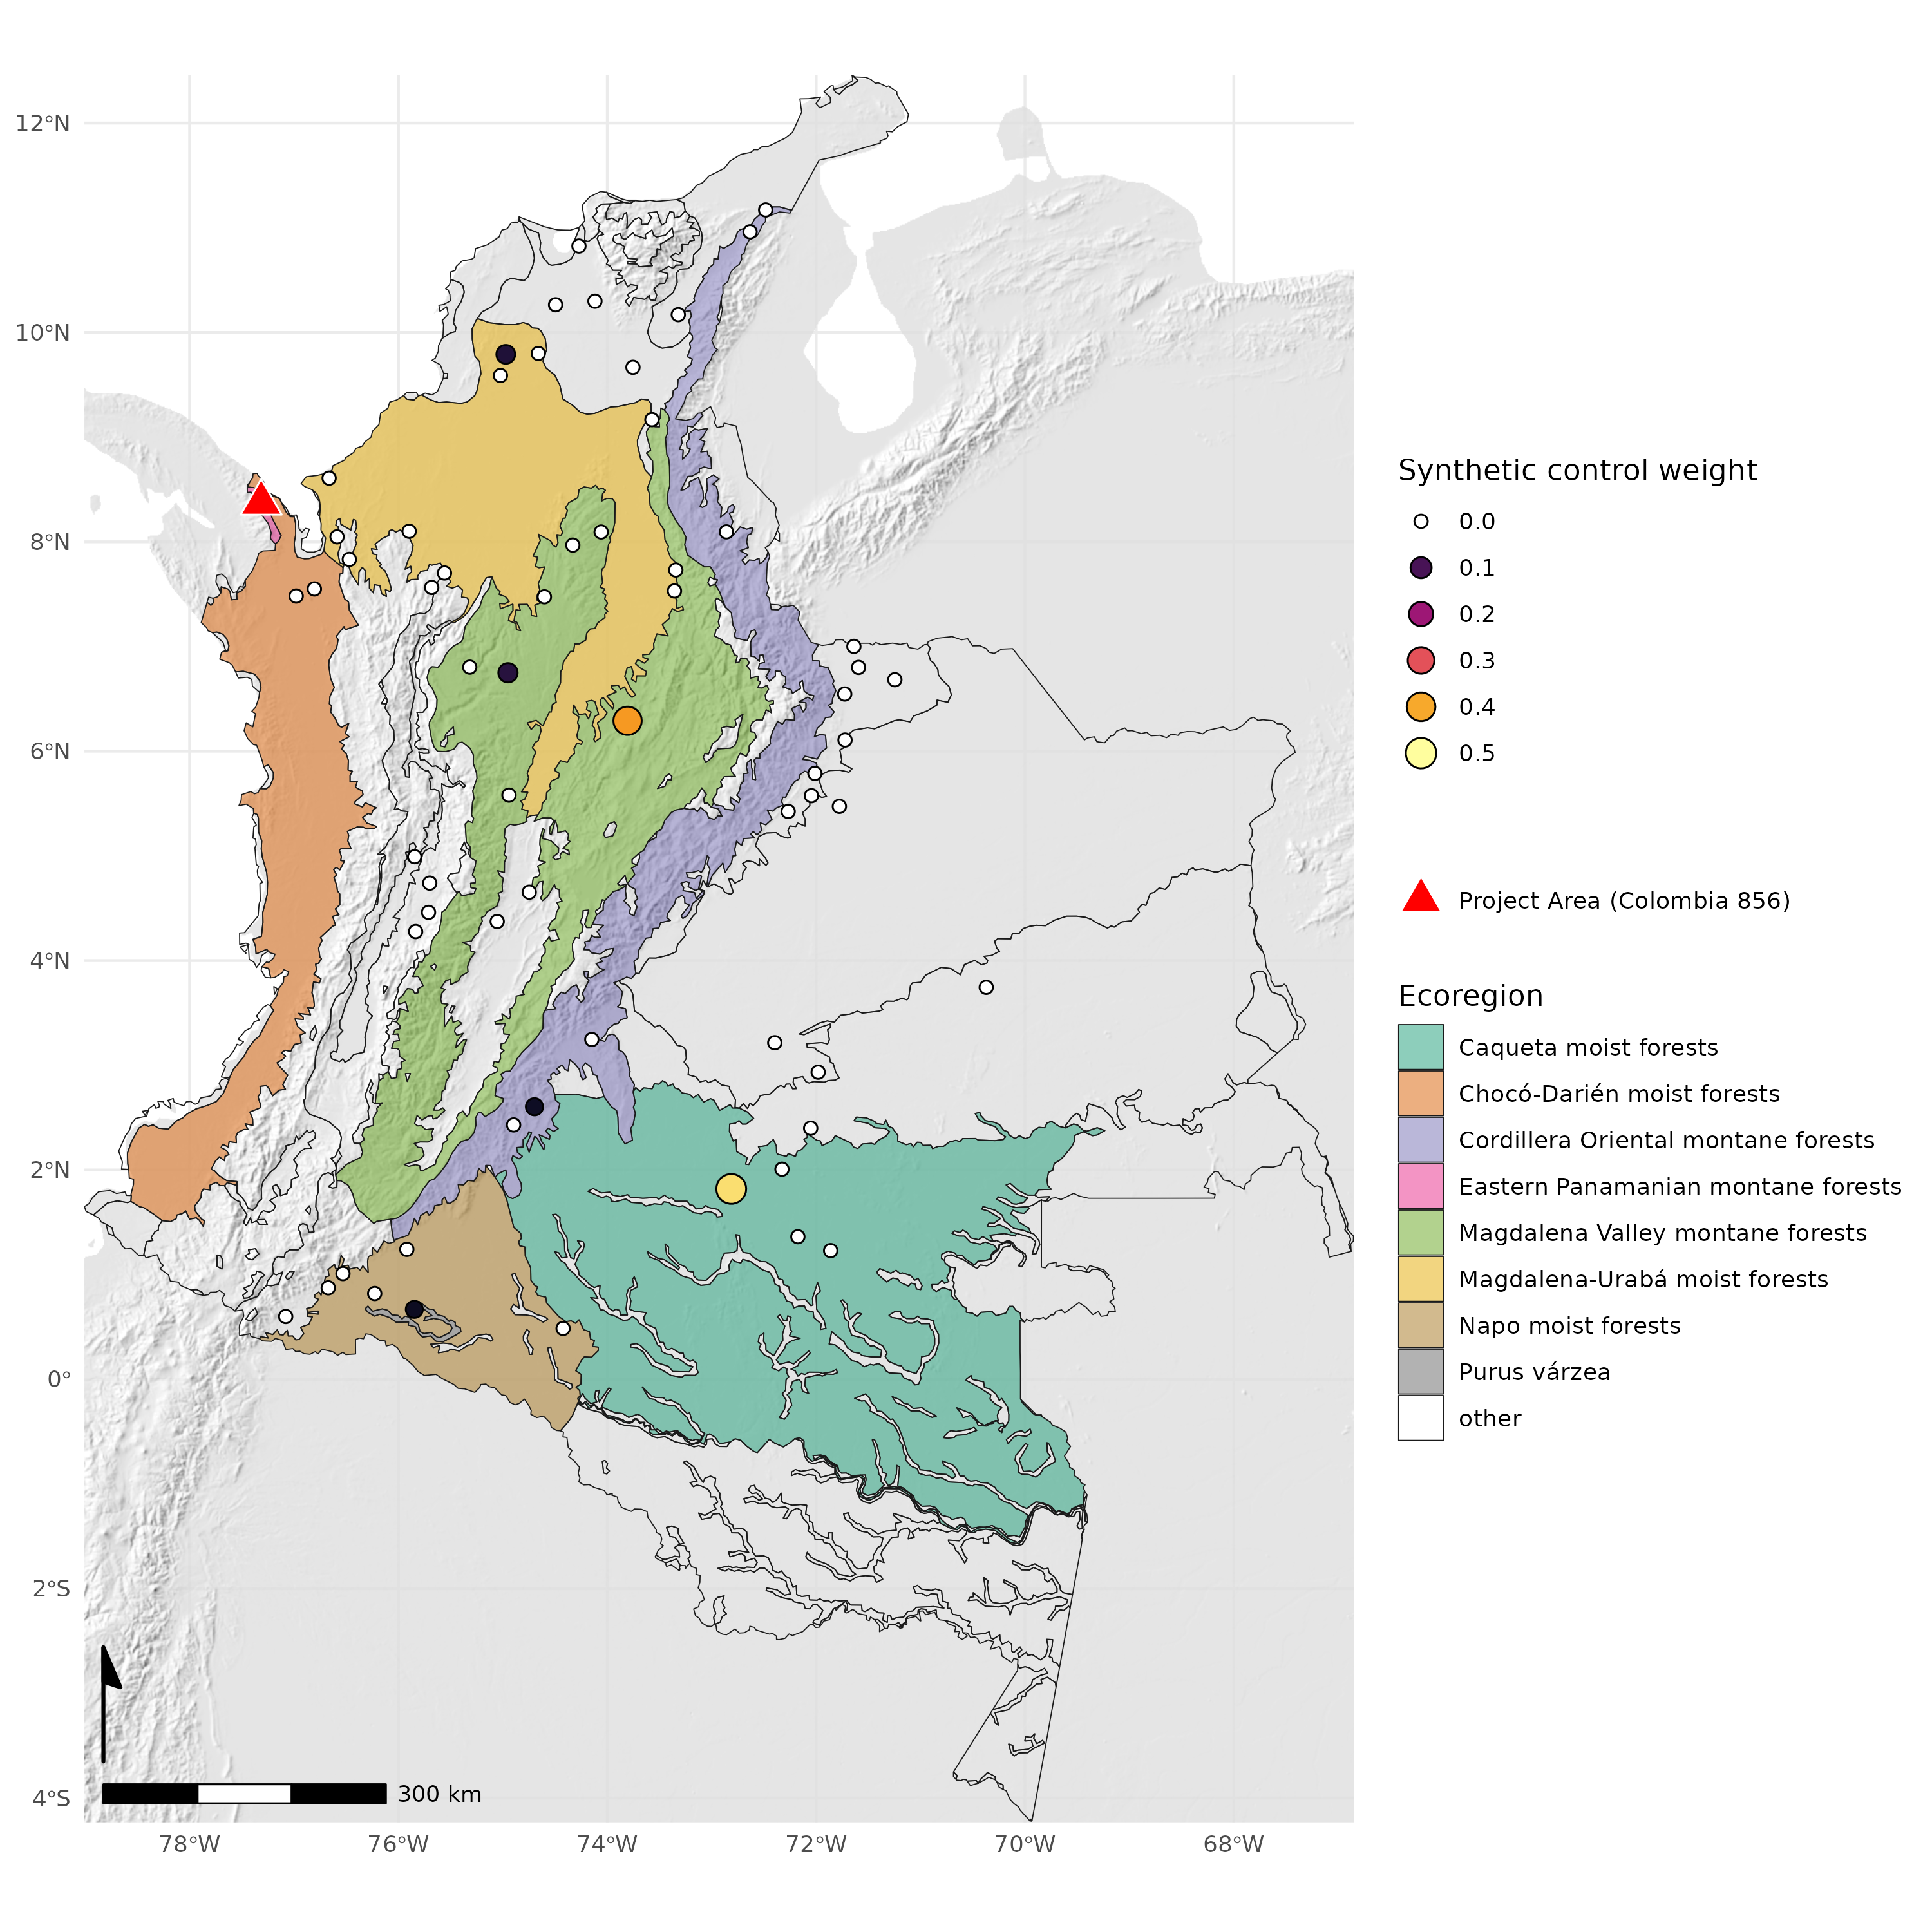
\includegraphics{figures/colombia_856_donors.png}

}

\caption{\label{fig-map}Map of the donor pool and their weighted
contribution to the Synthetic Control for Project-856. The project is
located to the north of Colombia's Choco Department, in the Darien
Mountain range and comprises a transition from lowland to montane
rainforest. Also presented are ecoregions
\citep{dinerstein_ecoregion-based_2017} that intersect weighted donors.
Project-856 was selected because it was the only one where fully
reproducible code was made available. To see interactive maps of this
and all other projects please see
\url{https://permian-global-research.github.io/science-letter-west-et-al/}.
Elevation data from https://registry.opendata.aws/terrain-tiles.}

\end{figure}

\newpage{}

\hypertarget{references}{%
\section{References}\label{references}}

\renewcommand{\bibsection}{}
\bibliography{bibliography.bib}




\end{document}
